%%% Preamble starts here.
\documentclass{amsart}
%for the heading
\usepackage{fancyhdr, enumerate}
%for the picture. 
\usepackage{tikz, calc}
%for importing images
\documentclass{article}
\usepackage{graphicx}
\usepackage{float}


%adjust the page width
\usepackage[margin=1in]{geometry}

%% The next line says how the "vertex" style of nodes should look: drawn as small circles.
\tikzstyle{vertex}=[circle, draw, inner sep=0pt, minimum size=6pt]
%%
%% Next, we make a \vertex command as a shorthand in place of \node[vertex} to get that style.
\newcommand{\vertex}{\node[vertex]}

\linespread{1.1}


%special commands for number sets
\def\RR{{\mathbb R}}
\def\NN{{\mathbb N}}
\def\ZZ{{\mathbb Z}}
\def\QQ{{\mathbb Q}}
\def\CC{{\mathbb C}}

% header
\lhead{\sc  Senior Seminar: Homework 2}
\chead{\sc Stefano Fochesatto } 
\rhead{due: Friday 01/24/2020}
\cfoot{}
\pagestyle{fancy}

%%%% Main document starts here.

\begin{document}
\thispagestyle{fancy}
 
\begin{enumerate}
%%%first problem
\item Prove or disprove: For any simple graph $G$, $\chi(G) \geq \delta(G),$ where $\delta(G)$ denotes the minimum degree of $G.$\\

\textbf{Answer:} Let $G$ be a $K_{3,3}$,
\begin{figure}[H]
\caption{Complete bipartite graph on 3 vertices.}
\centering
\includegraphics[width=\textwidth/4]{"Bipartite K3".png}
\end{figure}
Note that the blue and pink two coloring indicates that $\chi(G) \leq 2$ and since showing that $\chi(G) \neq 1$ is trivial we know that $\chi(G) = 2$ . By the definition of complete bipartite graph we know that $\delta(K_{m,n}) = min\{m,n\}$,  so therefore $\delta(G) = 3$. 

	\vspace{0.25in}
	
\item (1.1.5) Prove or disprove: If every vertex of a simple graph $G$ has degree 2, then $G$ must contain a cycle.\\

\textbf{Proof}(Contradiction:) Suppose a simple graph $G$ has degree 2, and that $G$ is acyclic. Now consider the longest path $l$ in $G$, with end vertices $a$ and $z$. Since each vertex in graph $G$ has degree 2 and $G$ is acyclic, vertices $a$ and $z$ must both be adjacent to vertices not contained inside the path $l$. Therefore $l$ is both the longest path and not the longest path. 
	
	\vspace{0.25in}
	
\item (1.1.16) Determine whether the graphs below are isomorphic. (Full credit will be given only for succinct solutions.)\\

\begin{center}
\begin{tabular}{lr}
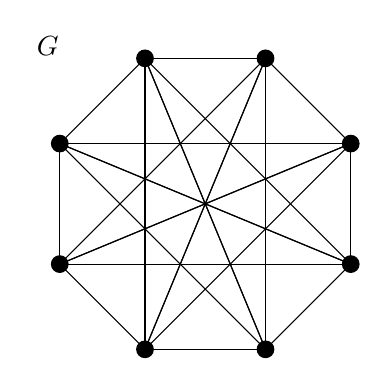
\begin{tikzpicture}
%name
\node at (-2,2){$G$};
%vertices
\foreach \i in {0,1,2,...,7}{
	\vertex[fill=black] (v\i) at (45*\i+22.5:2cm){};} 
%edges
\foreach \i in {0, 45, 90, ..., 315}{
	\draw (\i+22.5:2cm) -- (\i+67.5:2cm);
	\draw (\i+22.5:2cm) -- (\i+135+22.5:2cm);
	\draw (\i+22.5:2cm) -- (\i+180+22.5:2cm);}
\end{tikzpicture}
\quad 
&
\quad
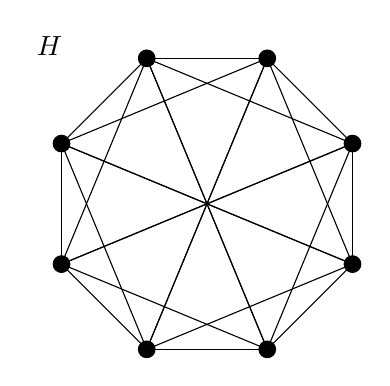
\begin{tikzpicture}
%name
\node at (-2,2){$H$};
%vertices
\foreach \i in {0,1,2,...,7}{
	\vertex[fill=black] (v\i) at (45*\i+22.5:2cm){};} 
%edges
\foreach \i in {0, 45, 90, ..., 315}{
	\draw (\i+22.5:2cm) -- (\i+67.5:2cm);
	\draw (\i+22.5:2cm) -- (\i+90+22.5:2cm);
	\draw (\i+22.5:2cm) -- (\i+180+22.5:2cm);}
\end{tikzpicture}\\
\end{tabular}
\end{center}

\textbf{Answer:} Consider the compliment of each graph, 

\begin{figure}[H]
\caption{Compliment of graphs G and H.}
\centering
\includegraphics[width=\textwidth]{"Ismorphosm".png}
\end{figure}

We can see that the compliment of $G$ is composed of 2 disconnected four cycles and  the compliment of $H$ is an 8 cycle. Thus the compliments of graphs $G$ and $H$ are not isomorphic and therefore there cannot exists an edge preserving, vertex bijection between $G$ and $H$, i.e $G$ and $H$ cannot be isomorphic.



	
	\vspace{0.25in}
	
\item (1.1.26) Let $G$ be a graph of girth 4 in which every vertex has degree $n$. Prove that $G$ has at least $2n$ vertices. Determine all such graphs with exactly $2n$ vertices.\\

\textbf{Answer:} Suppose a graph $G$ with girth 4, where every vertex has degree $n$. Now consider vertex $i$ in $G$. Note that vertex $i$ must be adjacent to $n$ other vertices, which themselves, cannot be adjacent to each other, in order to avoid a 3 cycle. We can fill in the rest of graph $G$ by making each vertex that is adjacent to $i$ also adjacent to $n-1$ vertices that are not adjacent to $i$. We do this to avoid a 3 cycle and to give each vertex degree $n$. Note, that what we have described is a complete bipartite graph $K_{n,n}$ which has girth 4 when $n \geq 2$ and each vertex has degree $n$. Since graph $G$ must be a complete bipartite graph, if each vertex has degree $n$ there must be at least $2n$ vertices.

 	\vspace{0.25in}
\end{enumerate}


\end{document}	

\item Let $G$ be the graph drawn below. Labels have been added for ease of reference.\\

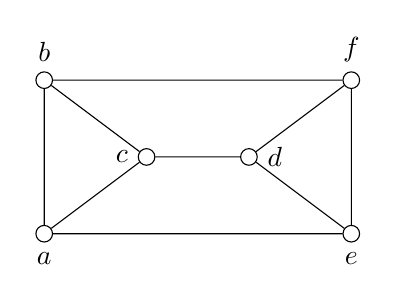
\begin{tikzpicture}[scale=1.3]
\vertex (A) at (0,0)[label=below:$a$]{};
\vertex (B) at (0,1.5)[label=above:$b$]{};
\vertex (C) at (1,0.75)[label=left:$c$]{};
\vertex (D) at (2,0.75)[label=right:$d$]{};
\vertex (E) at (3,0)[label=below:$e$]{};
\vertex (F) at (3,1.5)[label=above:$f$]{};
\draw (A) -- (B) -- (C) -- (A) (C) -- (D) -- (E) -- (F) --(D);
\draw (A) -- (E) (B) -- (F);
\end{tikzpicture}

	\begin{enumerate}
	\item Draw (using Tikz) $\overline{G}.$\\
	
	\textbf{Answer:}
	
	\vspace{0.25in}
	
	\item Determine $\chi(G)$ and prove your answer is correct.  (Note that I have helped by copying the graph below and showing how to add color.)\\
	
	\textbf{Answer:} Your answer may reference a picture ....

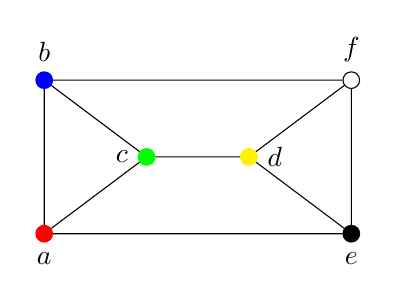
\begin{tikzpicture}[scale=1.3]
\vertex[fill, color=red] (A) at (0,0)[label=below:$a$]{};
\vertex[fill, color=blue] (B) at (0,1.5)[label=above:$b$]{};
\vertex[fill, color=green] (C) at (1,0.75)[label=left:$c$]{};
\vertex[fill, color=yellow] (D) at (2,0.75)[label=right:$d$]{};
\vertex[fill, color=black] (E) at (3,0)[label=below:$e$]{};
\vertex (F) at (3,1.5)[label=above:$f$]{};
\draw (A) -- (B) -- (C) -- (A) (C) -- (D) -- (E) -- (F) --(D);
\draw (A) -- (E) (B) -- (F);
\end{tikzpicture}

	
	\vspace{0.25in}
	
	\item Draw (using Tikz) a disconnected subgraph of $G.$\\
	
	\textbf{Answer:}
	
	\vspace{0.25in}
	
	\item Draw (using Tikz) a graph on 5 vertices that is \emph{not} a subgraph of $G.$\\
	
	\textbf{Answer:} 	
	
	
	\vspace{0.25in}
	
	\item Determine the length of a longest path in $G$ and justify your answer.\\
	
	\textbf{Answer:}
	
	\vspace{0.25in}
	
	\item Determine the length of a longest cycle in $G$ and justify your answer.\\
	
	\textbf{Answer:}
	
	\vspace{0.25in}
	
	\end{enumerate}
	
\item (problem 1.1.11) Determine the maximum size of a clique and the maximum size of an independent set in the graph below.\\

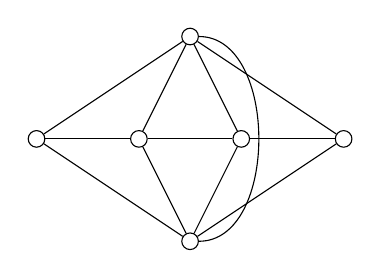
\begin{tikzpicture}[scale=1.3]
\vertex (a) at (1.5,1){};
\vertex (b) at (1.5,-1){};
\foreach \i in {0,1,2,3}{
	\vertex (v\i) at (\i,0){};
	\draw (a) -- (v\i) -- (b);
	}
\draw (v0)--(v1)--(v2)--(v3);
\draw (a) edge[bend left=90]  (b);
\end{tikzpicture}

\textbf{Answer:}
	
	\vspace{0.25in}	


\end{enumerate}
\end{document}